\documentclass[a4paper, 12pt]{article}

%%% Работа с русским языком
\usepackage{cmap}					% поиск в PDF
\usepackage{mathtext} 				% русские буквы в формулах
\usepackage[T2A]{fontenc}			% кодировка
\usepackage[utf8]{inputenc}			% кодировка исходного текста
\usepackage[russian]{babel}	% локализация и переносы

%%% Дополнительная работа с математикой
\usepackage{amsmath,amsfonts,amssymb,amsthm,mathtools} % AMS
\usepackage{icomma} % "Умная" запятая: $0,2$ --- число, $0, 2$ --- перечисление

%% Номера формул
%\mathtoolsset{showonlyrefs=true} % Показывать номера только у тех формул, на которые есть \eqref{} в тексте.

%% Шрифты
\usepackage{euscript}	 % Шрифт Евклид
\usepackage{mathrsfs} % Красивый матшрифт

%% Поля
\usepackage[left=2cm,right=2cm,top=2cm,bottom=2cm,bindingoffset=0cm]{geometry}

%% Русские списки
\usepackage{enumitem}
\makeatletter
\AddEnumerateCounter{\asbuk}{\russian@alph}{щ}
\makeatother

%%% Работа с картинками
\usepackage{graphicx}  % Для вставки рисунков
\graphicspath{{images/}{images2/}}  % папки с картинками
\setlength\fboxsep{3pt} % Отступ рамки \fbox{} от рисунка
\setlength\fboxrule{1pt} % Толщина линий рамки \fbox{}
\usepackage{wrapfig} % Обтекание рисунков и таблиц текстом

%%% Работа с таблицами
\usepackage{array,tabularx,tabulary,booktabs} % Дополнительная работа с таблицами
\usepackage{longtable}  % Длинные таблицы
\usepackage{multirow} % Слияние строк в таблице

%% Красная строка
\setlength{\parindent}{2em}

%% Интервалы
\linespread{1}
\usepackage{multirow}

%% TikZ
\usepackage{tikz}
\usetikzlibrary{graphs,graphs.standard}

%% Верхний колонтитул
\usepackage{fancyhdr}
\pagestyle{fancy}

%% Перенос знаков в формулах (по Львовскому)
\newcommand*{\hm}[1]{#1\nobreak\discretionary{}
	{\hbox{$\mathsurround=0pt #1$}}{}}

%% Мои дополнения
\usepackage{float} %Добавляет возможность работы с командой [H] которая улучшает расположение на странице
\usepackage{gensymb} %Красивые градусы
\usepackage{graphicx}               % Импорт изображений
\usepackage{caption} % Пакет для подписей к рисункам, в частности, для работы caption*

% подключаем hyperref (для ссылок внутри  pdf)
\usepackage[unicode, pdftex]{hyperref}

%%% Теоремы
\theoremstyle{plain}                    % Это стиль по умолчанию, его можно не переопределять.
\renewcommand\qedsymbol{$\blacksquare$} % переопределение символа завершения доказательства

\newtheorem{theorem}{Теорема}[section] % Теорема (счетчик по секиям)
\newtheorem{proposition}{Утверждение}[section] % Утверждение (счетчик по секиям)
\newtheorem{definition}{Определение}[section] % Определение (счетчик по секиям)
\newtheorem{corollary}{Следствие}[theorem] % Следстиве (счетчик по теоремам)
\newtheorem{problem}{Задача}[section] % Задача (счетчик по секиям)
\newtheorem*{remark}{Примечание} % Примечание (можно переопределить, как Замечание)
\newtheorem{lemma}{Лемма}[section] % Лемма (счетчик по секиям)

\begin{document}
    \newcommand{\HRule}{\rule{\linewidth}{0.7mm}} % Defines a new command for the horizontal lines, change thickness here
	
	\begin{center}
		\large\textbf{Московский Физико-Технический Институт}\\ % Name of your university/college
		\large\textbf{(государственный университет)}
	
		\vfill
		
		\Large Лабораторная работа по курсу общей физики № *labnum*\\[0.5cm] % Preambule of your document title
		
		
		\HRule
		\\[0.4cm]
		{ \huge \bfseries *name of your labwork*}% Title of your document
		\\[0.4cm] 
		\HRule
		\\[0.5cm]
		
		\ \\
	\textbf{\large Автор:} \\	
	\large *your name* *groupname*\\ % Your name and something more, your group num for example
		\vfill
		\hspace*{-0.8 cm}
\includegraphics[width=100 pt]{frkt_logo}\\ % logo of your  company/university/college
		\large Долгопрудный, 2021 % location and year
	\end{center}

\newpage
\setcounter{page}{2}
\fancyfoot[c]{\thepage}
\fancyhead[L] {Работа № *labnum*} % some information in page header
\fancyhead[R]{}

    \section*{Цель работы}

    \section*{Теоретическая чать}

    \subsection*{Частица над потенциальной ямой}

    Запишем уравнения Шредингера в общем виде

    \begin{equation}
        -\frac{\hbar^2}{2mc} \psi'' + U \psi = E \psi
    \end{equation}

    \[ \psi'' + \frac{2mc}{\hbar^2}(E - U) \psi = 0 \]

    Рассмотрим потенциальную яму глубиной $U_0$ и шириной $l$.

    \begin{figure}
        \centering
        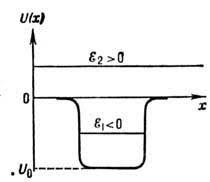
\includegraphics[scale=1]{ph.jpeg}
        \caption{Потенциальная яма}
        \label{fig:ph}
    \end{figure}

    Тогда для области вне ямы уравнение запишется

    \begin{equation}
        \psi'' + \frac{2mc}{\hbar^2} E = 0
    \end{equation}

    где $E$ -- потенциальная энергия частицы. А для области внутри ямы уравнение запишем

    \begin{equation}
        \psi'' + \frac{2mc}{\hbar^2}(E + U_0) = 0
    \end{equation}

    Введем коэффициенты

    \begin{equation}
        k_1^2 = \frac{2mc}{\hbar^2} E
    \end{equation}

    \begin{equation}
        k_2^2 = \frac{2mc}{\hbar^2}(E + U_0)
    \end{equation}

    Приведем качественное объяснение эффекта Рамзауэра.

    Запишем коэффициент прохождения частицы через потенциальную яму

    \begin{equation}
        D = \frac{16 k_1^2 k_2^2}{16 k_1^2 k_2^2 + 4(k_1^2 - k_2^2) \sin^2 (k_2 l)}
    \end{equation}

    Как мы видим, коэффициент прохождения частицы зависит от $\sin^2 (k_2 l)$, а $k_2$ в свою очередь зависит от энергии
    частицы. Именно поэтому при разных энергиях частиц зависимость прохождения частицы над потенциальной ямой разная и имеет
    последовательность минимумов и максимумов. В частности, коэффициент прохождения максимальный, при условии

    \begin{equation}
        k_2 l = \sqrt{\frac{2mc}{\hbar^2}(E + U_0)} l = \pi n ~~ (n = 1, 2, \dots)
    \end{equation}

    Теперь приведем более прикладное объяснение.

    Перейдем от волновых функций частиц к их длинам волн. Частице с энергией $E$ соответсвует длина волны де Бройля

    \begin{equation}
        \lambda = \frac{h}{\sqrt{2mE}}
    \end{equation}

    При прохождении частицы над потенциальной ямой длина волны меняется:

    \begin{equation}
        \lambda' = \frac{h}{\sqrt{2m(E+U_0)}}
    \end{equation}

    Яму в этом случае можно рассматривать в качестве оптически более плотной среды. В таком случае можно рассмотреть
    интерференцию прошедшей и отраженной волн

    \begin{figure}
        \centering
        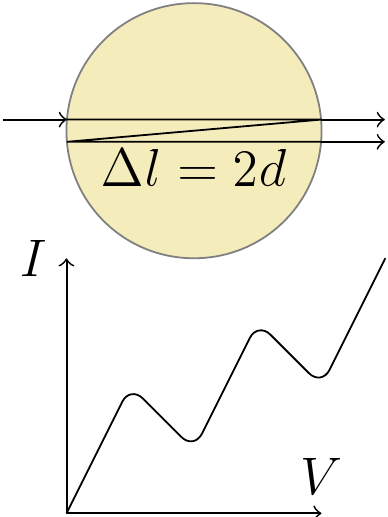
\includegraphics[scale=0.5]{Ramsauer.png}
        \caption{Интерференция волн}
        \label{fig:interf}
    \end{figure}

    Запишем условие на максимум и минимум, $\Delta$ -- оптическая разность хода. Условие на максимум: оптическая разность хода
    равна целому числу полуволн

    \begin{equation}
        \Delta = 2l = 2n \frac{\lambda'}{2} = n \lambda'
    \end{equation}

    Условие на минимум: оптическая разность хода равна полуцелому числу полуволн

    \begin{equation}
        \Delta = 2l = (2n + 1) \lambda'
    \end{equation}

    Таким образом, подставляя в формулы выражения для волны де Бройля, получаем

    \begin{equation}
        \begin{cases}
            2l = \sqrt{\frac{h^2}{2m (E_1 + U_0)}} \\
            2l = \frac{3}{2} \sqrt{\frac{h^2}{2m (E_2 + U_0)}} \\
        \end{cases}
    \end{equation}

    где $E_1$ -- энергия частиц, дающая максимум, $E_2$ -- энергия частиц, дающая минимум, $U_0$ -- глубина потенциальной ямы.

    Решая совместно эти 2 уравнения можно исключить $U_0$ и найти ширину ямы

    \begin{equation} \label{eq:width}
        l = \sqrt{\frac{5 h^2}{32 m (E_2 - E_1)}}
    \end{equation}

    а так же расчитать глубину ямы

    \begin{equation} \label{eq:U_0}
        U_0 = \frac{4}{5}E_2 - \frac{9}{5}E_1
    \end{equation}

    В нашем эксперементе кинетическую энергию частица получает, при прохождении ускоряющей разности потенциалов $E = e V$, 
    где $V$ -- ускоряющая разность потенциалов. Поэтому

    \[ E_1 = e V_1 ~~~ E_2 = e V_2 \]

    \subsection*{Расчет погрешностей}

    Расчитаем погрешности для формул \eqref{eq:width} и \eqref{eq:U_0}.

    По правилу вычисления косвенных погрешностей

    \begin{equation}
        \varepsilon_l = \sqrt{\varepsilon_{E_1}^2 + \varepsilon_{E_2}^2} \Rightarrow \sigma_l = \sqrt{\varepsilon_{E_1}^2 + \varepsilon_{E_2}^2} l
    \end{equation}

    Аналогично

    \begin{equation}
        \varepsilon_{U_0} = \sqrt{\varepsilon_{E_1}^2 + \varepsilon_{E_2}^2} \Rightarrow \sigma_{U_0} = \sqrt{\varepsilon_{E_1}^2 + \varepsilon_{E_2}^2} U_0
    \end{equation}

    \section*{Эксперементальная установка}

    \section*{Обработка эксперементальных данных}
    % m = 9.1 * 10^{-31} кг
    % 1 эВ = 1.6 * 10^{-19} дж
    % h = 2pi * 6.58 * 10^{-16} эВ*с

    С помощью осцилографа выведем на экран вольт амперную характиристику и измерим $E_1$ и $E_2$
    для двух различных напряжений накала $V_1 = 2.89$ В и $V_2 = 2.60$ В.

    На обоих напряжениях накала $E_1$ и $E_2$ оказались одинаковыми: $E_1 = (2 \pm 0.01)$ В, $E_2 = (7.2 \pm 0.01)$ В.
    Исходя из этих величин и пользуясь формулами \eqref{eq:width} и \eqref{eq:U_0} посчитаем 

    \begin{center}
        $l = (3.00 \pm 0.02)$ \AA \\
        $U_0 = (2.16 \pm 0.01)$ эВ \\
    \end{center}

    Теперь снимем вольт амперную характиристику в статическом режиме для тех же значений напряжений накала.
    Результаты приведем в таблице \ref{tab:data}.

    \begin{table}[]
    \centering
    \begin{tabular}{|ll|ll|ll|}
    \hline
    \multicolumn{2}{|l|}{4 В}                                      & \multicolumn{2}{l|}{6 В}                                     & \multicolumn{2}{l|}{9 В}                                     \\ \hline
    \multicolumn{1}{|l|}{V$\pm 0.01$, В}    & I $\pm 0.001$ мА     & \multicolumn{1}{l|}{V$\pm 0.01$, В}    & I $\pm 0.001$ мА    & \multicolumn{1}{l|}{V$\pm 0.01$, В}    & I $\pm 0.001$ мА    \\ \hline
    \multicolumn{1}{|l|}{4.25}              & 0.062                & \multicolumn{1}{l|}{2.60}              & 0.019               & \multicolumn{1}{l|}{5.28}              & 0.015               \\ \hline
    \multicolumn{1}{|l|}{6.25}              & 0.094                & \multicolumn{1}{l|}{6.05}              & 0.066               & \multicolumn{1}{l|}{10.0}              & 0.090               \\ \hline
    \multicolumn{1}{|l|}{8.14}              & 0.127                & \multicolumn{1}{l|}{9.12}              & 0.120               & \multicolumn{1}{l|}{12.6}              & 0.133               \\ \hline
    \multicolumn{1}{|l|}{10.8}              & 0.171                & \multicolumn{1}{l|}{12.3}              & 0.169               & \multicolumn{1}{l|}{14.9}              & 0.167               \\ \hline
    \multicolumn{1}{|l|}{14.6}              & 0.223                & \multicolumn{1}{l|}{16.0}              & 0.221               & \multicolumn{1}{l|}{17.4}              & 0.203               \\ \hline
    \multicolumn{1}{|l|}{17.5}              & 0.258                & \multicolumn{1}{l|}{16.7}              & 0.228               & \multicolumn{1}{l|}{19.5}              & 0.228               \\ \hline
    \multicolumn{1}{|l|}{17.9}              & 0.262                & \multicolumn{1}{l|}{17.4}              & 0.239               & \multicolumn{1}{l|}{20.7}              & 0.235               \\ \hline
    \multicolumn{1}{|l|}{18.7}              & 0.269                & \multicolumn{1}{l|}{18.1}              & 0.249               & \multicolumn{1}{l|}{21.6}              & 0.236               \\ \hline
    \multicolumn{1}{|l|}{19.7}              & 0.274                & \multicolumn{1}{l|}{19.1}              & 0.258               & \multicolumn{1}{l|}{22.5}              & 0.233               \\ \hline
    \multicolumn{1}{|l|}{21.0}              & 0.274                & \multicolumn{1}{l|}{20.0}              & 0.263               & \multicolumn{1}{l|}{24.0}              & 0.203               \\ \hline
    \multicolumn{1}{|l|}{21.9}              & 0.271                & \multicolumn{1}{l|}{21.0}              & 0.263               & \multicolumn{1}{l|}{24.3}              & 0.183               \\ \hline
    \multicolumn{1}{|l|}{22.3}              & 0.261                & \multicolumn{1}{l|}{21.9}              & 0.257               & \multicolumn{1}{l|}{24.5}              & 0.098               \\ \hline
    \multicolumn{1}{|l|}{22.7}              & 0.251                & \multicolumn{1}{l|}{22.5}              & 0.252               & \multicolumn{1}{l|}{25.2}              & 0.078               \\ \hline
    \multicolumn{1}{|l|}{23.0}              & 0.221                & \multicolumn{1}{l|}{23.2}              & 0.236               & \multicolumn{1}{l|}{26.5}              & 0.071               \\ \hline
    \multicolumn{1}{|l|}{23.3}              & 0.211                & \multicolumn{1}{l|}{23.4}              & 0.221               & \multicolumn{1}{l|}{27.6}              & 0.077               \\ \hline
    \multicolumn{1}{|l|}{24.3}              & 0.213                & \multicolumn{1}{l|}{23.5}              & 0.205               & \multicolumn{1}{l|}{28.8}              & 0.093               \\ \hline
    \multicolumn{1}{|l|}{24.7}              & 0.218                & \multicolumn{1}{l|}{23.8}              & 0.169               & \multicolumn{1}{l|}{29.6}              & 0.112               \\ \hline
    \multicolumn{1}{|l|}{25.4}              & 0.232                & \multicolumn{1}{l|}{24.8}              & 0.144               & \multicolumn{1}{l|}{30.6}              & 0.138               \\ \hline
    \multicolumn{1}{|l|}{26.3}              & 0.249                & \multicolumn{1}{l|}{25.8}              & 0.152               & \multicolumn{1}{l|}{31.6}              & 0.160               \\ \hline
    \multicolumn{1}{|l|}{26.8}              & 0.259                & \multicolumn{1}{l|}{27.7}              & 0.194               & \multicolumn{1}{l|}{33.8}              & 0.207               \\ \hline
    \multicolumn{1}{|l|}{27.6}              & 0.275                & \multicolumn{1}{l|}{29.0}              & 0.220               & \multicolumn{1}{l|}{35.8}              & 0.240               \\ \hline
    \multicolumn{1}{|l|}{28.5}              & 0.293                & \multicolumn{1}{l|}{29.9}              & 0.240               & \multicolumn{1}{l|}{37.0}              & 0.250               \\ \hline
    \multicolumn{1}{|l|}{29.4}              & 0.309                & \multicolumn{1}{l|}{31.9}              & 0.277               & \multicolumn{1}{l|}{38.6}              & 0.255               \\ \hline
    \multicolumn{1}{|l|}{32.1}              & 0.359                & \multicolumn{1}{l|}{33.4}              & 0.306               & \multicolumn{1}{l|}{39.4}              & 0.253               \\ \hline
    \multicolumn{1}{|l|}{33.8}              & 0.389                & \multicolumn{1}{l|}{35.0}              & 0.333               & \multicolumn{1}{l|}{41.1}              & 0.241               \\ \hline
    \multicolumn{1}{|l|}{35.0}              & 0.409                & \multicolumn{1}{l|}{36.9}              & 0.346               & \multicolumn{1}{l|}{42.9}              & 0.229               \\ \hline
    \multicolumn{1}{|l|}{37.3}              & 0.419                & \multicolumn{1}{l|}{39.0}              & 0.347               & \multicolumn{1}{l|}{44.4}              & 0.218               \\ \hline
    \multicolumn{1}{|l|}{38.5}              & 0.419                & \multicolumn{1}{l|}{40.9}              & 0.330               & \multicolumn{1}{l|}{46.4}              & 0.201               \\ \hline
    \multicolumn{1}{|l|}{39.4}              & 0.411                & \multicolumn{1}{l|}{42.9}              & 0.316               & \multicolumn{1}{l|}{48.2}              & 0.196               \\ \hline
    \multicolumn{1}{|l|}{40.5}              & 0.400                & \multicolumn{1}{l|}{44.5}              & 0.308               & \multicolumn{1}{l|}{50.1}              & 0.192               \\ \hline
    \multicolumn{1}{|l|}{40.9}              & 0.395                & \multicolumn{1}{l|}{46.1}              & 0.305               & \multicolumn{1}{l|}{51.7}              & 0.199               \\ \hline
    \multicolumn{1}{|l|}{41.7}              & 0.391                & \multicolumn{1}{l|}{47.7}              & 0.308               & \multicolumn{1}{l|}{52.7}              & 0.204               \\ \hline
    \multicolumn{1}{|l|}{42.7}              & 0.387                & \multicolumn{1}{l|}{49.4}              & 0.317               & \multicolumn{1}{l|}{}                  &                     \\ \hline
    \multicolumn{1}{|l|}{44.5}              & 0.388                & \multicolumn{1}{l|}{51.6}              & 0.330               & \multicolumn{1}{l|}{}                  &                     \\ \hline
    \multicolumn{1}{|l|}{45.2}              & 0.390                & \multicolumn{1}{l|}{53.1}              & 0.343               & \multicolumn{1}{l|}{}                  &                     \\ \hline
    \multicolumn{1}{|l|}{49.4}              & 0.417                & \multicolumn{1}{l|}{56.0}              & 0.370               & \multicolumn{1}{l|}{}                  &                     \\ \hline
    \end{tabular}
    \caption{Таблица эксперементальных данных для трех запирающих напряжений}
    \label{tab:data}
    \end{table}

    По эксперементальным данным построим графики вольт амперных характиристику \ref{fig:V1}, \ref{fig:V2}, \ref{fig:V1vsV2}.

    \begin{figure}
        \centering
        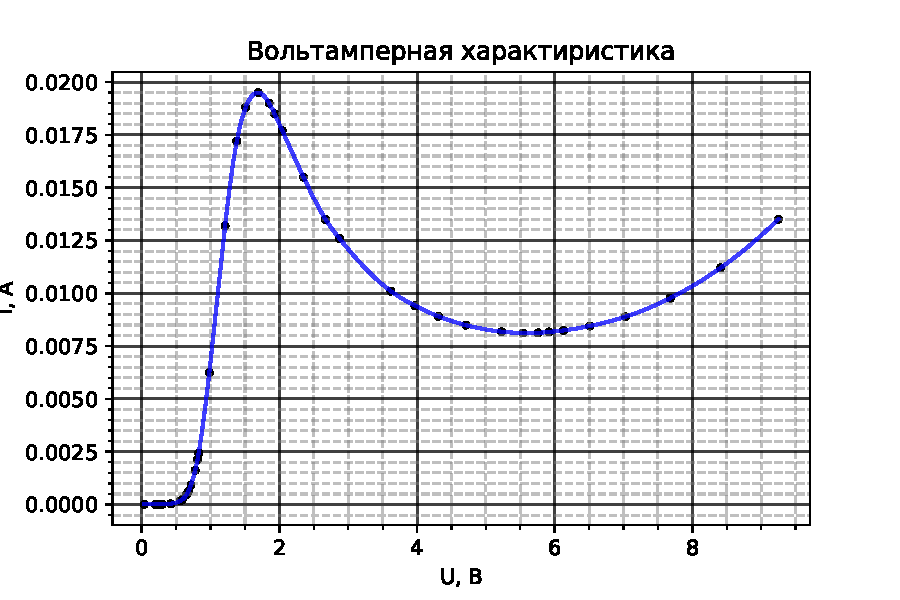
\includegraphics[width=\textwidth]{graph1.pdf}
        \caption{Воль амперная характиристика для $V_1 = 2.98$ В}
        \label{fig:V1}
    \end{figure}

    \begin{figure}
        \centering
        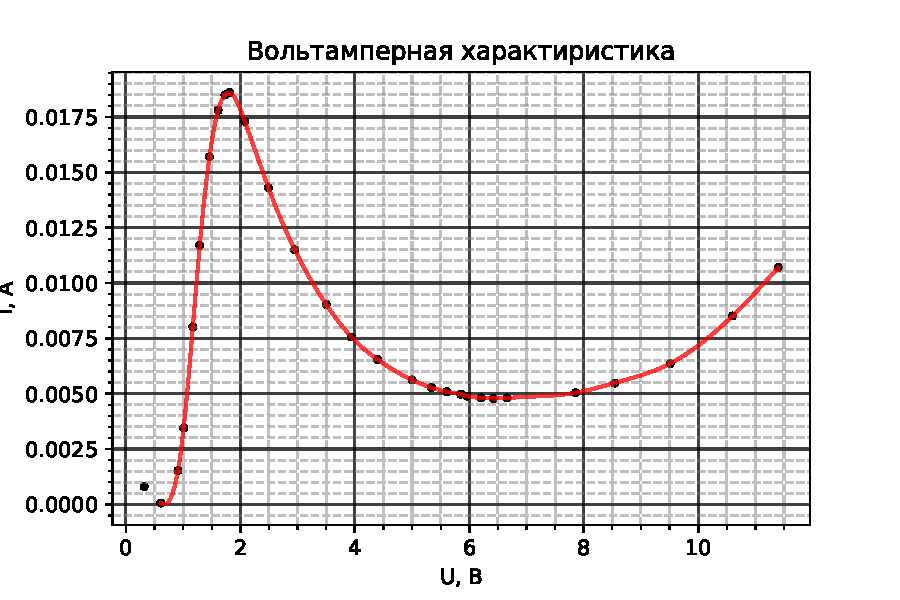
\includegraphics[width=\textwidth]{graph2.pdf}
        \caption{Воль амперная характиристика для $V_2 = 2.60$ В}
        \label{fig:V2}
    \end{figure}

    \begin{figure}
        \centering
        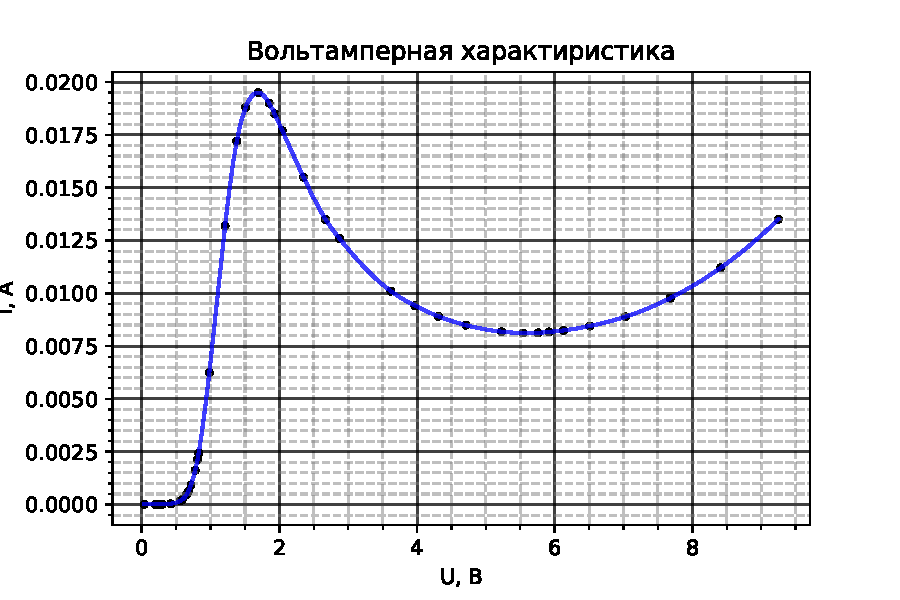
\includegraphics[width=\textwidth]{graph3.pdf}
        \caption{Сравнение вольт амперных характиристик}
        \label{fig:V1vsV2}
    \end{figure}

    По графикам найдем $E_1$ и $E_2$ для каждого значения запирающего напряжения и расчитаем $l$.

    \begin{table}[]
    \centering
    \begin{tabular}{|c|c|c|c|c|}
    \hline
      & $V$    & $U_{min}$ & $U_{max}$ & $\sigma_U$ \\ \hline
    1 & 2.98   & 5.54      & 1.69      & 0.01       \\ \hline
    2 & 2.60   & 6.42      & 1.81      & 0.01       \\ \hline
    \end{tabular}
    \caption{Результаты по статическому режиму}
    \label{tab:static_mod}
\end{table}

    Таким образом

    \begin{center}
        Для $V_1 = 2.98$ В \\ $l = (3.49 \pm 0.02)$ \AA, $U_0 = (1.39 \pm 0.01)$ эВ \\[0.5 cm]
        Для $V_2 = 2.60$ В \\ $l = (3.19 \pm 0.02)$ \AA, $U_0 = (1.88 \pm 0.01)$ эВ \\[0.5 cm]
    \end{center}

    Кроме того, учитывая, что $w \sim \ln I_a$ где $w$ -- вероятность рассеяния электрона в зависимости от энергии, а $I_a$ --
    так анода, можем построить качественную зависимость изменения $w$. \textbf{Примечание:} поскольку известны не все величины,
    график отражает лишь качественную зависимость. Численные значения не отражают действительность!

    \begin{figure}
        \centering
        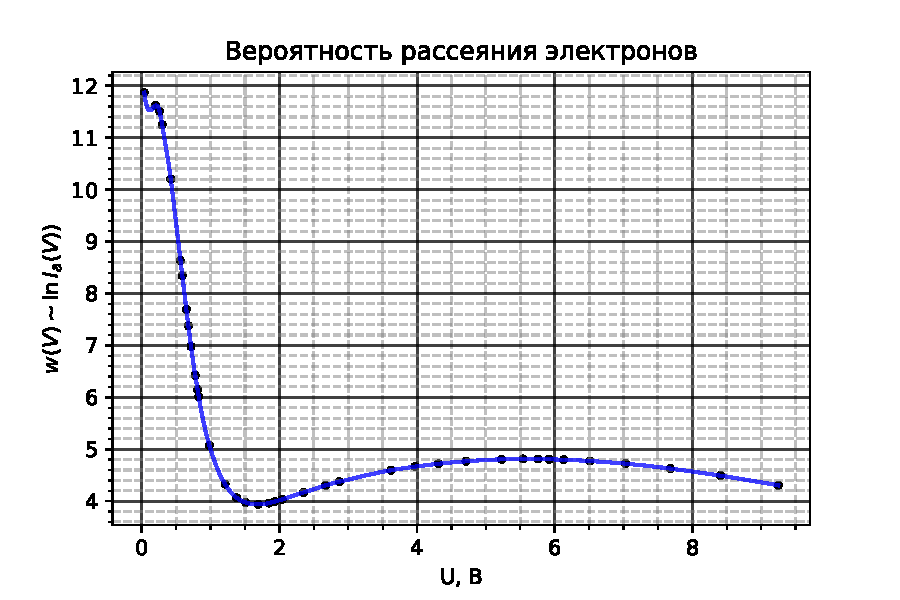
\includegraphics[]{graph4.pdf}
        \caption{Качественный график зависимости вероятности рассеяния электронов от их энергии}
        \label{fig:graph4}
    \end{figure}

    Найдем, при каком значении ускоряющего потенциала на вольт амперной характиристике мы увидили бы максимумы более высоких
    порядков (начиная со второго и так далее). Воспользуемся для этого формулой на дифрационный максимум

    \begin{equation}
        2 l = n \frac{h}{\sqrt{2m (E - U_0)}}
    \end{equation}

    из нее получаем

    \begin{equation}
        U \sim E = \frac{n^2 h^2}{8 l^2 m} - U_0
    \end{equation}

    Для расчета возмем значения $l$ и $U_0$ для напряжения $V_2 = 2.60$ В, поскольку при этом напряжении величина $l$ наиболее
    близка к табличной. Результаты расчетов представлены в таблице.

    \begin{table}[]
    \centering
    \begin{tabular}{|c|c|}
    \hline
    $n$ & $U$, В     \\ \hline
    1   & 1.81       \\ \hline
    2   & 12.89      \\ \hline
    3   & 31.36      \\ \hline
    4   & 57.22      \\ \hline
    \end{tabular}
    \caption{Значения напряжений для максимумов ВАХ}
    % \label{}
\end{table}

    \section*{Вывод}

    В данной работе мы получили вольт амперную характиристику на тиратроне в статическом и динамическом режимах.
    По графикам мы убедились в справедливости эффекта Рамзауэра, что подтверждает волновую природу элетронов. Используя 
    данные мы расчитали ширину потенциальной ямы (для атома ксенона), а так же ее глубину. Полученная в ходе эксперемента
    величина $l$ довольно близка к табличному значению $l = 280$ пм, но все же отличается от нее. Это связано с тем, что
    мы использовали упрощенную модель прямоугольной потенциальной ямы, что в реальности вообще говоря является достаточно грубым
    приближением.

\end{document}